\documentclass[a4paper]{article}

\usepackage{listings}
\usepackage{graphicx}
\usepackage{caption}
\usepackage{subcaption}
\usepackage{fancyhdr}
\usepackage{color}
\usepackage{xcolor}
\usepackage[hidelinks]{hyperref}
\pagestyle{fancy}

\addtolength{\oddsidemargin}{-.875in}
\addtolength{\evensidemargin}{-.875in}
\addtolength{\headwidth}{1.75in}
\addtolength{\textwidth}{1.75in}

\lhead{Clarke-Wright Implementation}
\rhead{SET09117}
\lfoot{Report}
\cfoot{\thepage}
\rfoot{Gareth Pulham, 40099603}

\lstdefinestyle{customc}{
    belowcaptionskip=1\baselineskip,
    frame=single,
    breaklines=true,
    xleftmargin=\parindent,
    language=C,
    showstringspaces=false,
    basicstyle=\footnotesize\ttfamily,
    keywordstyle=\bfseries\color{green!40!black},
    commentstyle=\itshape\color{purple!40!black},
    identifierstyle=\color{blue},
    stringstyle=\color{orange},
}

\begin{document}
    \begin{titlepage}
        \title{Algorithms and Data Structures Coursework: An Implementation of the Clarke-Wright Route Optimisation in C}
        \author{Gareth Pulham, 40099603}
        \date{\today}
        \maketitle
        \thispagestyle{empty}
        \begin{abstract}
            As part of Napier University's Algorithms and Data Structures class (SET09117), students were tasked to implement and report upon an implementation
            of the Clarke-Wright \cite{CW} route optimisation algorithm. This document will cover one such implementation by student 40099603, covering how it was
            tested and how it performs in comparison to naive 1-route-per-customer routes.
        \end{abstract}
    \end{titlepage}

    \tableofcontents

    \section{Introduction}
    Vehicle routing is a classic algorithmic challenge, with a long history both theoretical and practical in nature.
    Identifying optimal routes has serious implications to the cost of business operations, and as such has been widely researched by delivery companies,
    such as UPS, Fedex, and others, because of this.
    In computer science, the best known form is the Travelling Salesman Problem, to which references date back at least as far as 1832. Computer science
    research into this field is particularly common in undergraduate studies as it offers a hands-on introduction to graph theory.

    One instance of research into the Vehicle Routing Problem field is the 1964 paper ``Scheduling of Vehicles from a Central Depot to a Number of Delivery Points''
    by Clarke and Wright \cite{CW}, which puts forward the so called ``Savings Method''. In this method, all delivery points are given a designated route of their
    own, the highest cost scenario for a multi-route delivery operation. Following this, all possible permutations of route merges are calculated and ranked
    biggest saving to worst. Given two delivery points $i$ and $j$, the saving that can be made is $ S_{ij} = c_{j0} + c_{0i} - c_{ij} $, as derived by
    Lysgaard \cite{Lysgaard} in ``Clarke and Wright's Savings Algorithm''. Once all these merge savings have been ranked, they are applied where possible. 
    Thanks to the ranking, the biggest saving route merges have the highest likelyhood of being applicable.

    In this case, the implementation of the algorithm was completed in C, and as will be shown to have the strengths and weaknesses that this language tends towards.
    Notably, the solution is very fast in comparison to most comparable implementations in other languages, such as Java and Python, as memory management is
    manually and carefully considered, as well as being able to take advantage of C's fast native maths support.
    Some limitations include:
    \begin{itemize}
        \item All coordinates (both customer and depot) must be within the range of the platforms \texttt{int} type
        \item All customer loads and depot truck sizes must be within the range of the platforms \texttt{int} type
        \item Performance is highly dependent on memory management speeds and pointer comparison speeds
    \end{itemize}
    Many of the limitations are tunable, for example, larger coordinate ranges can be permitted by adjusting the types used in \texttt{ClarkeWright.h} and
    \texttt{ClarkeWright.c}.

    \section{Method}
    As part of the algorithm implementation, the developer was mindful of the following test points:
    \begin{itemize}
        \item Correctness - the generated routes should cover all customers, and never exceed additional constraints such as delivery vehicle size.
        \item Speed and efficiency - the algorithm should run quickly and scale well with input size.
        \item Relative improvement - that is, the level of improvement over naive 1-route-per-customer routes.
    \end{itemize}
    These points were all tested in an automated and repeatable fashion across a wide dataset, ranging from 10 to 1000 customers.

        \subsection{Correctness}
        As part of the work, a tool, \texttt{Verify.jar} was provided that ensured that all customers in a given CSV file had been serviced, and that no
        routes generated ever exceeded the additional restraints. This tool additionally calculated the cost of the routes produced.

        \subsection{Speed and efficiency}
        The use of the algorithm in the test code was instrumented to measure the CPU time consumed between starting and finishing the algorithm,
        and the number of milliseconds consumed is printed during runtime. The algorithm was run multiple times over each test data instance, including
        cache warming pre-runs, and their run times recorded. From these records, we can calculate the average runtime.

        \subsection{Relative improvement}
        A stub version of the algorithm was also executed that produced naive 1-route-per-customer routes. These routes were also tested by \texttt{Verify.jar}
        and their costs recorded for comparison with the complete algorithm.
    

    \section{Results}
        \subsection{Correctness}
        For this algorithm, the primary correctness requirements were that all customers \emph{must} be delivered to and that all routes \emph{must} have a lower
        total load than the delivery vehicles capacity. Failure to adhere to these requirements in every route would be considered a failed implementation, as it
        does not correctly solve the problem. To test this, \texttt{Verify.jar} should be called with the problem CSV and the possible solution CSV
        as arguments. The output will be either a pass or fail, and in each case more information is produced such as the total cost of a valid solution, or the
        missing customers or overloaded route if the solution was invalid.

        \begin{figure}[h]
            \centering
            \begin{subfigure}{.5\textwidth}
                \centering
                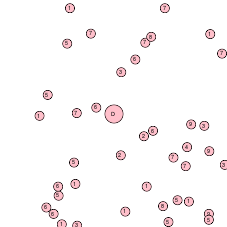
\includegraphics[width=.4\linewidth]{images/40-customers-blank.png}
                \caption{SVG file produced for an unrouted problem}
                \label{fig:sub1}
            \end{subfigure}%
            \begin{subfigure}{.5\textwidth}
                \centering
                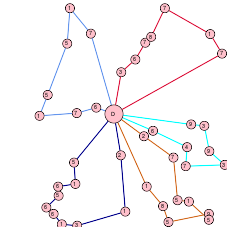
\includegraphics[width=.4\linewidth]{images/40-customers-routed.png}
                \caption{SVG file produced for a routed problem}
                \label{fig:sub1}
            \end{subfigure}
            \caption{\texttt{Verify.jar} SVG outputs showing unrouted problem and valid routed solution}
            \label{fig:correctness}
        \end{figure}
        
        \texttt{Verify.jar} shown that for all test problems, valid solutions were produced. While this does not prove the algorithms implementation correct,
        for the purposes of this work, these outputs satisfy our test for correctness.
        
        \subsection{Speed and efficiency}
        An additional area of investigation is the speed and efficiency of the algorithm. The test code in \texttt{main.c} that calls the implementation also
        records the CPU time consumed by the algorithm for reporting after the solution is calculated. The results are shown below.
        % Put the graph in here
        
        \begin{minipage}{\textwidth}
            \centering
            \begin{tabular}{ c c }
                Number of customers & Average runtime (milliseconds) \\
                \hline
                \hline
                10                  &  0.00569 \\
                20                  &  0.02419 \\
                30                  &  0.05222 \\
                40                  &  0.10364 \\
                50                  &  0.17757 \\
                60                  &  0.18564 \\
                70                  &  0.28376 \\
                80                  &  0.41329 \\
                90                  &  0.45694 \\
                100                 &  0.65025 \\
                200                 &  2.74443 \\
                300                 &  6.21002 \\
                400                 &  8.22210 \\
                500                 & 14.17183 \\
                600                 & 22.50074 \\
                700                 & 29.85135 \\
                800                 & 38.22703 \\
                900                 & 48.18592 \\
                1000                & 62.10673 \\
                \hline
            \end{tabular}
        \end{minipage}
        
        \subsection{Relative improvement}
        The purpose of the algorithm is to provide efficient routes. In this test, we compare the cost of our implementation vs. the cost of a naive
        1-route-per-customer solution.
        
        \begin{figure}[h]
            \centering
            \begin{subfigure}{.5\textwidth}
                \centering
                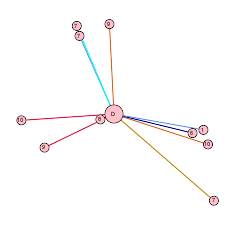
\includegraphics[width=.4\linewidth]{images/10-customers-naive.png}
                \caption{SVG file produced for a naive solution}
                \label{fig:sub1}
            \end{subfigure}%
            \begin{subfigure}{.5\textwidth}
                \centering
                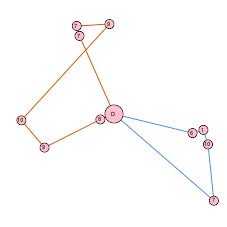
\includegraphics[width=.4\linewidth]{images/10-customers-routed.png}
                \caption{SVG file produced for a solution by our implementation of C\&W}
                \label{fig:sub1}
            \end{subfigure}
            \caption{\texttt{Verify.jar} SVG outputs showing solutions from naive and our implementation of C\&W}
            \label{fig:speedandefficiency}
        \end{figure}
        
        \begin{minipage}{\textwidth}
            \centering
            \begin{tabular}{ c c c c }
                Number of customers & Cost (naive) & Cost (C\&W) & Improvement (\%) \\
                \hline
                \hline
                10                  &   3781       &  1471       & 156 \\
                20                  &   7930       &  2374       & 233 \\
                30                  &  10302       &  3251       & 216 \\
                40                  &  15775       &  3393       & 364 \\
                50                  &  20072       &  4687       & 328 \\
                60                  &  23193       &  5063       & 358 \\
                70                  &  25924       &  5049       & 413 \\
                80                  &  28756       &  6218       & 362 \\
                90                  &  34580       &  6909       & 400 \\
                100                 &  38703       &  7529       & 414 \\
                200                 &  76928       & 12968       & 493 \\
                300                 & 116480       & 16958       & 586 \\
                400                 & 153608       & 22644       & 578 \\
                500                 & 188739       & 27996       & 574 \\
                600                 & 228961       & 33416       & 585 \\
                700                 & 266674       & 37265       & 615 \\
                800                 & 311675       & 42246       & 637 \\
                900                 & 347699       & 48802       & 612 \\
                1000                & 390783       & 51398       & 660 \\
                \hline
            \end{tabular}
        \end{minipage}

    \section{Conclusion}
    Clarke and Wright's algorithm is designed to lower the costs of multi-route vehicle routing. As shown in the above test results, the implementation of this
    algorithm can result in large savings, up to over 600\% in some cases, with increasing gains as the number of delivery points increases.

    In all the requirement areas (correctness, speed and efficiency, and relative improvement), the implementation of this algorithm has shown strong results.
    Future work could focus on improving the performance of the algorithm - in particular, the sorting of potential savings can be slow, especially as the lower
    end of the savings list are increasingly less important due to small impact and the decreasing likelyhood that the savings can be applied at all.

    Ultimately, the developer considers this implementation and its writeup a success - across the board, challenges were identified, challenged, and defeated,
    and in the process, a working solution was completed and demonstrated. Following the submission deadline, the developer intends to engage in peer review
    with other developers, learning from other implementations and receiving feedback on their own, if permitted by markers.

    \bibliographystyle{abbrv}
    \bibliography{report}
    
    \section{Appendices}
        \subsection{Full table of results for speed and efficiency testing}
        \subsection{Source code listings}
            This section contains the listings for functional code in this implementation of the Clarke-Wright algorithm.
            Complete versions of the entire project, including test data, build files, and the source for this report will be available from
            \url{https://github.com/AbstractBeliefs/ADS-Coursework-2015/} after the submission deadline (Saturday 21st November 2015, 23:55).
            \subsubsection{main.c}
                \lstinputlisting[style=customc]{../src/main.c}
            \subsubsection{ClarkeWright.h}
                \lstinputlisting[style=customc]{../src/ClarkeWright.h}
            \subsubsection{ClarkeWright.c}
                \lstinputlisting[style=customc]{../src/ClarkeWright.c}
        \subsection{Test code listings}
            \subsubsection{NaiveStub.c}
                \lstinputlisting[style=customc]{NaiveStub.c}
            \subsubsection{test\_costs.py}
                \lstinputlisting{../test_tools/test_costs.py}
            \subsubsection{test\_times.sh}
                \lstinputlisting{../test_tools/test_times.sh}
\end{document}
